\chapter{Preliminaries: Isabelle}\label{chapter:preliminaries}
\section{Isabelle/Scala and Isabelle/ML}
Isabelle is implemented in two main programming languages: \textit{Scala} and 
\textit{Standard ML}.
In the context of Isabelle, these are however referred to as 
\textit{Isabelle/Scala} and \textit{Isabelle/ML}, since the code style is
tied tightly to Isabelle. The 
\textit{Isabelle/Isar Implementation} manual describes Isabelle/ML as a 
``certain
culture based on Standard ML. Thus it is not a new programming language, but a
certain way to use SML at an advanced level within the Isabelle environment.''\cite{isabelle-implementation}.

The two implementation languages play different roles in Isabelle.
\textit{The Isabelle System Manual} highlights this difference by 
comparing them to \textit{mathematics} and \textit{physics}:
Isabelle/ML corresponds to implementing the tools for the mathematics of 
Isabelle (like tactics or proofs), whereas Isabelle/Scala is for
physics, i.e., to interface with other tools and systems of the
``outside world'' like IDEs \cite{isabelle-system}.

\section{The PIDE Document model}
\textit{Isabelle/PIDE} stands for \textit{Prover IDE}, which is the framework
managing the editor, the prover, and other tools around the Isabelle
proof assistant \cite{wenzel2019interaction,isabelle-pide}. The document model is at the 
heart of the protocol: it decouples interactive exploration of the sources in the editor 
from the parallel processing of theories by the prover. Modifying the sources or scrolling
down the buffer creates new document \textit{versions}, which prompt the prover to
interrupt its processing or process the newly visible content as needed. The prover 
communicates its execution results through PIDE
XML markup over the input sources and through messages. 
The editor uses this information to provide semantic information about the sources through
syntax highlighting, underlines, and other GUI elements.
Decoupling rendering and editing from
the prover process is possible through document \textit{snapshots}, that represent
the state of the document at a particular time point \cite{wenzel2019interaction}.


The document model is how Isabelle/Scala and Isabelle/ML are
connected. The internal protocol is responsible for
communication between the two worlds, with the sources in Isabelle/Scala
imitating those in Isabelle/ML: there are many \texttt{.ML} files with
corresponding \texttt{.scala} counterparts to have the same 
abstraction in both implementation frameworks \cite{Wenzel2012}.

\section{Isabelle Syntax}
The Isabelle syntax is split into two parts as described in the
\textit{The Isabelle/Isar Reference Manual} \cite{isabelle-isar-ref}:
\begin{itemize}
    \item The \textit{Outer Syntax}, representing the \textit{theory} language.
    It covers the proofs, specifications, and outlines of theories.
    \item The \textit{Inner Syntax}, representing the \textit{term} language.
    It is used to specify types and logic terms. Inner syntax elements occur
    as atomic entities in the outer syntax elements.
\end{itemize}
\autoref{fig:syntax} shows the difference between the two syntax categories:
the text with a light-grey background corresponds to \textit{inner syntax},
the rest is \textit{outer syntax}.
\begin{figure}[htpb]
    \centering
    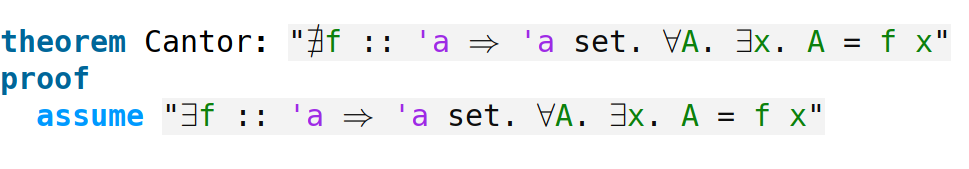
\includegraphics[width=0.7\textwidth]{images/syntax.png}
    \caption[Example Syntax]{Syntax example from HOL/Examples/Cantor.thy}\label{fig:syntax}
\end{figure}

\section{IDE Support}
The primary way to interact with Isabelle is through Isabelle/jEdit \cite{isabelle-jedit}. It is
the de facto IDE for Isabelle. It consists of the jEdit text editor with the Isabelle
plugin, which provides its own panels and functionalities. The main focus is
to enable asynchronous and parallel processing of documents. \textit{Dockable}
windows are a central part of the jEdit editor providing functionality beyond
editing text (like searching or exploring the document structure). They are heavily 
utilized in the Isabelle plugin to
extend the capabilities of the IDE, for example to display the prover messages
and command results in the \textit{Output} panel.

\begin{figure}[htpb]
    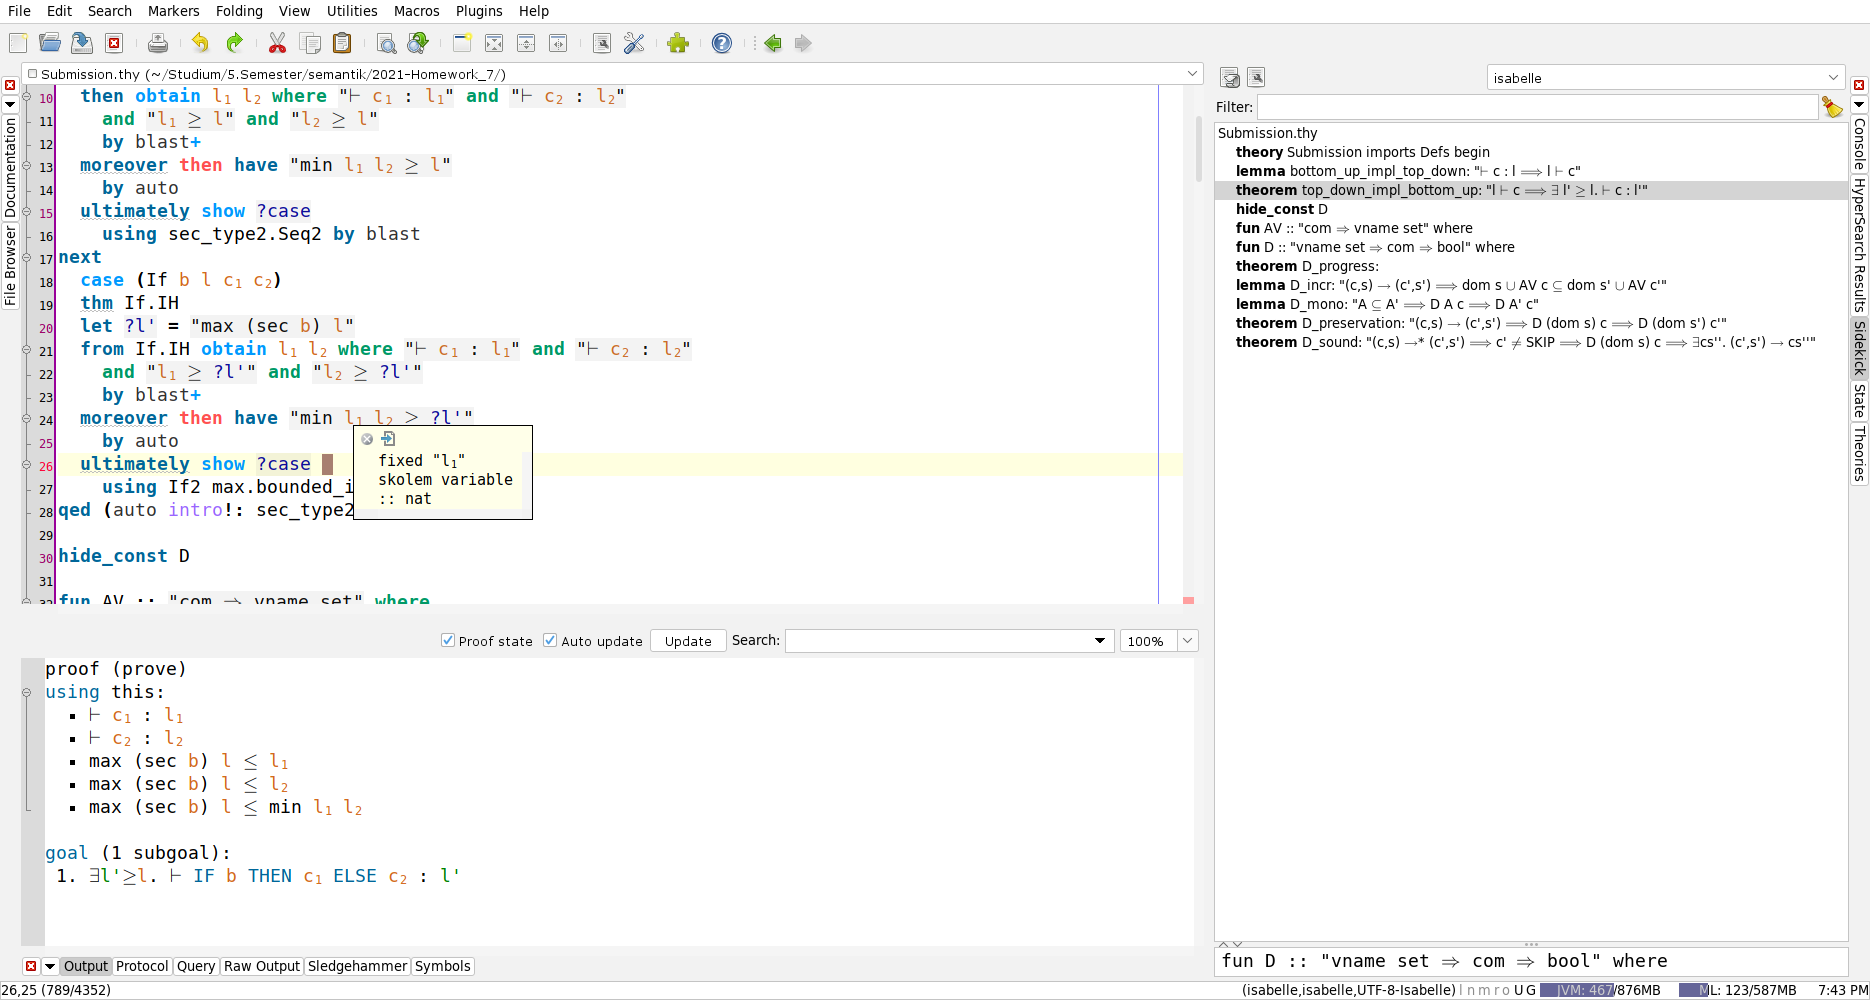
\includegraphics[width=\textwidth]{images/jedit-plain.png}
    \caption[Isabelle/jEdit in action]{Isabelle/jEdit in action}\label{fig:jedit-plain}
\end{figure}

Another editor that can be used with Isabelle is VSCode \footnote{\url{https://code.visualstudio.com/}} through the \textit{Isabelle/VSCode}
extension \cite{isabelle-pide}. It leverages Isabelle/PIDE for 
\textit{Language Server Protocol}\footnote{\url{https://microsoft.github.io/language-server-protocol/}} functionality. The \texttt{Isabelle-emacs} project
\footnote{\url{https://github.com/m-fleury/isabelle-emacs}} is
a similar implementation aiming to bring the same functionalities to emacs.